\part{Contexto da Empresa}

\chapter[Contexto da Empresa]{Contexto da Empresa}

O objetivo em questão é propor ao nosso cliente uma solução para seus problemas empresariais que possam ser resolvidos com a elaboração de algum sistema de software. O contexto de projeto será realizado dentro da Climacolândia Doces, da área alimentícia, uma pequena empresa localizada fisicamente na casa dos donos, em Brasília. Os principais mantenedores são um casal, que assumem todos os papéis dentro da empresa de acordo com suas capacidades.

O objetivo da empresa é confeccionar diversos tipos de doce, bolos, cupcakes, doces menores etc, para quaisquer ocasiões desejada pelo consumidor. Os produtos são feitos com base na necessidade de quem faz o pedido ou na criatividade do(a) doceiro(a).


\section{Organização da Empresa}

Geralmente uma empresa tem um esquema de organização com várias ramificações, mas cada tipo tem suas características individuais dependendo da sua área de atuação no mercado. O exemplo abaixo mostra sistema organizacional geral de uma empresa grande de doces.

%figura
\begin{figure}[h!]
	\centering
	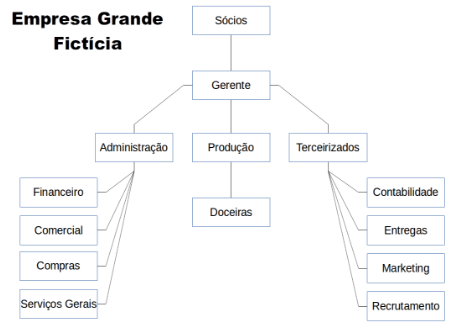
\includegraphics[scale=0.7]{figuras/grande.png}
	\caption{Sistema organizacional geral}
\end{figure}

A Climacolândia sendo uma empresa pequena mantida apenas por duas pessoas, possui um esquema de organização com baixa complexidade e bem menos ramificações. Os papéis são divididos para o casal de forma bastante flexível, onde alguns sendo fixos dependentes das habilidades individuais e outros alternados dependendo da situação momentânea de tempo. O exemplo abaixo mostra sistema organizacional da Climacolândia Doces, as pessoas serão definidas como Mantenedor A e Mantenedor B.

%figura
\begin{figure}[h!]
	\centering
	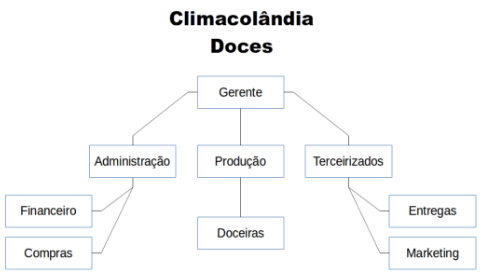
\includegraphics[scale=0.7]{figuras/climacolandia.png}
	\caption{Sistema organizacional da Climacolândia}
\end{figure}

\begin{itemize}
\item \textbf{Mantenedor A:} Gerente, Doceiro, Compras, Administração, Financeiro, Marketing e Produção.
\item \textbf{Mantenedor B:} Administração, Compras, Marketing, Entregas e Financeiro.
\end{itemize}

\section{Descrição do Problema}

Como a empresa possui apenas duas pessoas trabalhando, onde elas ainda atuam em outras áreas fora desse mercado durante determinado tempo do dia, as tarefas diárias designadas para os papéis dentro da empresa podem sobrecarregar o casal, principalmente o Mantenedor A, que mais cuida da parte financeira, produção e é ao mesmo tempo é o doceiro.

O uso de anotações em diários e cadernos é a metodologia adotada pela empresa para o controle de estoque e de vendas. Pode-se encontrar vários riscos com a utilização desse método, por exemplo, dependendo da quantidade de informação já guardada pela empresa, pode haver uma ocupação física exacerbada de cadernos, diários e folhas e futuramente pode-se haver também a perda dessas informações por conta de falta de organização no arquivamento desses materiais ou por danificamento dos mesmos.

Tendo como base a reunião com o cliente, percebeu-se que com a sobrecarga de tarefas e o modo de arquivamento de todo o andamento diário de trabalho, o maior problema encontrado é a perda de controle de toda a informação referente ao financeiro (vendas e gastos) e compras, onde a empresa necessita principalmente de um controle da quantia de lucro ao final das vendas e do controle de estoque que também interfere no financeiro. Eles possuem a necessidade também de saber o custo não só na compra dos materiais para a confecção dos doces como também saber os gastos em tempo de mão de obra na confecção do produto.

Outro problema, mas em menor escala, é ter uma otimização na área de marketing, onde a falta de tempo afeta nas atualizações dos meios de anúncio dos produtos vendidos.